% TO DO: quelle für text und bild hinzufügen
\section{Versuchsaufbau und Durchf\"uhrung}
Die Korrelation von Photonen eines NV-Zentrums kann mittels eines  Hanbury Brown-Twiss Interferometer
% paper als quelle fuer die erlaeuterungen einfuegen
gemessen werden. Eine schematische Skizze des Versuchsaufbaues ist in der Abbildung \ref{fig:Versuchsaufbau} dargestellt. 
Die mittlere Lebensdauer des angeregenten Zustandes in einem NV-Zentrum ist geringer, als die Todzeit einer Photodiode. 
Deshalb k\"onnen zwei aufeinander folgende Photonen nicht von der gleichen Photodiode gemessen werden. 
Dies ist aber notwendig, umd die Korrelation zu untersuchen. Aus diesem Grund, werden bei diesem Versuch 2 Photodioden benutzt. 
Zur Aufteilung des Strahles für die beiden Photodioden wird eine Strahlteiler benutzt. Zur Anregung der NV-Zentren wird ein Argon Laser benutzt. 
Die gewünschte Mode des Lasers kann mit Filtern herausgefiltert werden. Dazu gehören eine Pinhole, ein Polarisationsfilter und ein Frequnezfilter.  
Zum Ausw\"ahlen des gew\"unschten Bereiches des Diamanten, wird ein Piezoelement benutzt. 
Damit ist eine Verschiebung in allen drei Raumdimensionen m\"oglich, wobei eine Dimension stets fixiert werden muss und dann die anderen beiden variiert werden k\"onnen. 
Die Verschiebung ist notwendig, um f\"ur die Messung den gew\"unschten Bereich des Diamten, ein NV-Zentrum, auszuw\"ahlen. Gemessen wird die Zeitdifferenz, zwischen dem Eintreffen eines Photons an der einen Diode und eines Photons an der anderen Diode. 
Aufgetragen werden die gemessene Zeiten in einem Histogramm.   
\begin{figure}[H]
\centering
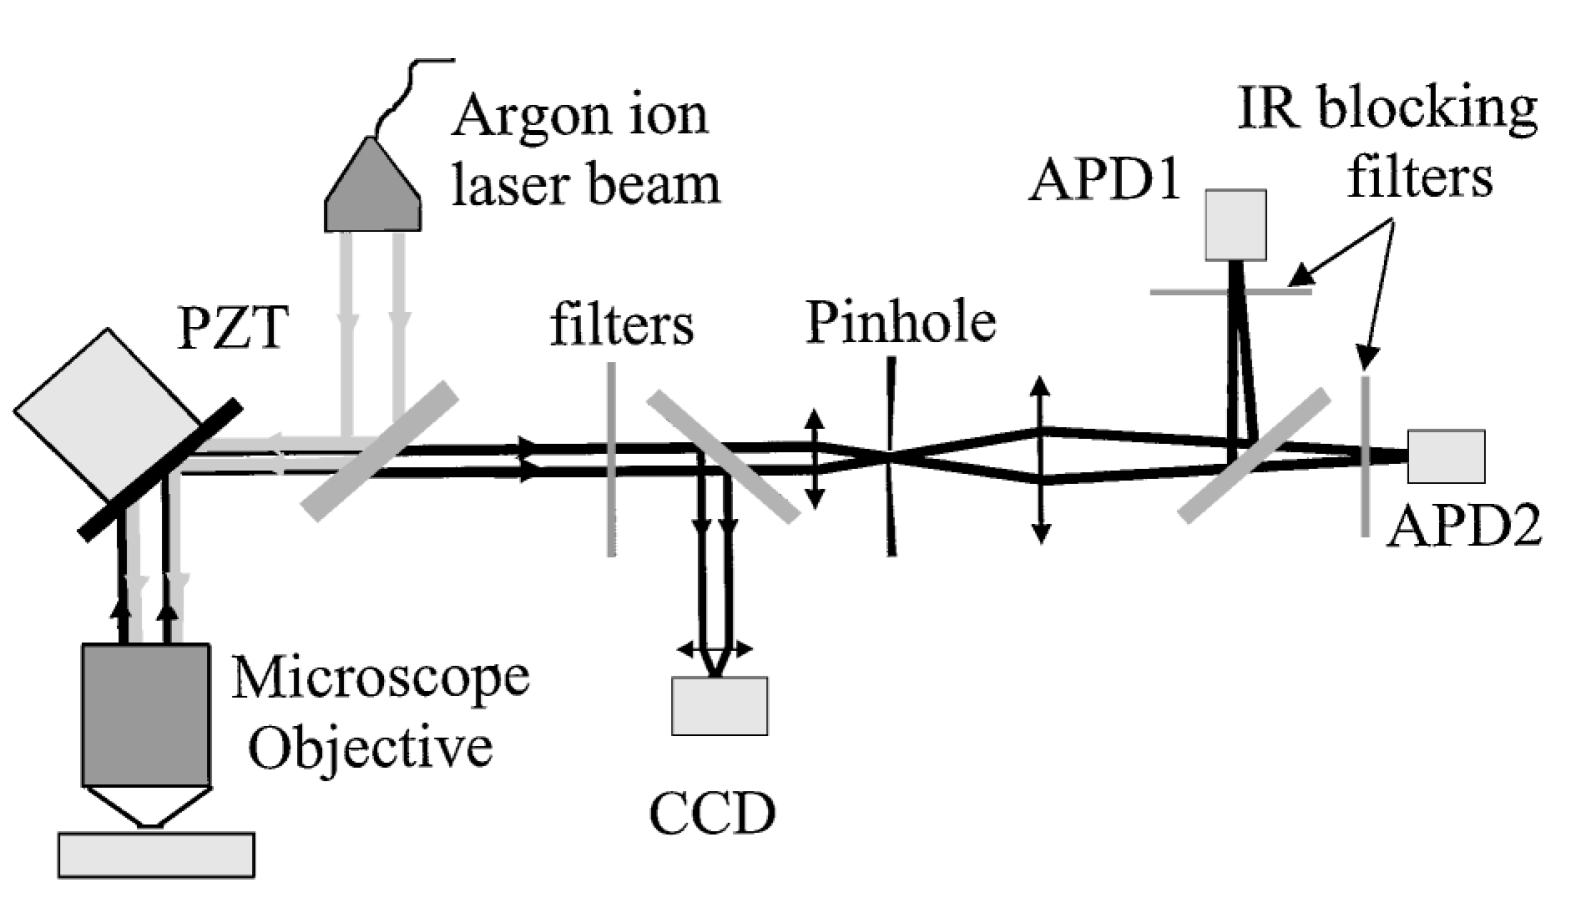
\includegraphics[scale=0.6]{Versuchsaufbau.PNG}
\caption{Schematischer Versuchsaufbau eines Hanbury Brown-Twiss-Setup zur Messung der Korrelation von Photonen von NV-Zentren.  }
\label{fig:Versuchsaufbau}
\end{figure}
Als erstes wird die y-Richtung festgehalten um den richigen Werte f\"uer die z-Richtung zu erhalten. 
Danach kann die z-Richtung festgehalten werden und die x-y-Ebene gemessen werden. 
F\"ur die Messung muss nun ein Bereich ausgew\"ahlt werden, in dem es  ein NV-Zentrum gibt.  
Dieser Bereich sollte in dem Histogramm f\"ur die x-y-Ebene eine engef\"ahr runde Form habe. 
Au{\ss}erdem darf der Bereich nicht zu gro{\ss} sein und es d\"urfen auch nicht zuviele Photonen aus diesem Bereich emitiert werden. 
Diese Kriterien sind notwendig, da eine Emission von Photonen in Diamaten auch andere Ursachen, zum Beispiel Fehlstellen, haben kann. 
Nach dem ein Breich f\"uer die Messung ausgew\"ahlt worden ist, muss der Autofokus aktiviert werden, damit ein Abdriften der gew\"unschten Stelle vermieden werden kann. Gemessen wird nun f\"ur dieses NV-Zentrum, die Zeitdifferenzen zwischen dem Eintreffen der Photonen an den beiden Photodioden. 
Diese Messung soll f\"ur zwei NV-Zentren durchgef\"uhrt werden. 
Um ausagekr\"aftige Resultatte zu erziehlen, soll jede Messung ungef\"ahr zwei Stunden lang dauern. 
Als drittes soll ein Gebiet des Diamanten gemessen werden, bei dem es sich nicht um ein NV-Zentrum handelt. 
Dazu soll ein Bereich ausgew\"ahlt werden, in dem ein Vielfaches der Photonen eines NV-Zentrums emittiert wird. Aufgrund der stärkeren Emission reicht eine viel kleinere Messdauer aus. 

%TO DO: bild aus paper einfuegen, mit quellenangabe

